\documentclass[12pt]{extarticle}
%Some packages I commonly use.
\usepackage[portuguese]{babel}
\usepackage{graphicx}
\usepackage{framed}
\usepackage[normalem]{ulem}
\usepackage{amsmath}
\usepackage{amsthm}
\usepackage{amssymb}
\usepackage{amsfonts}
\usepackage{enumerate}
\usepackage[utf8]{inputenc}
\usepackage{float}
\usepackage{gensymb}
\usepackage[top=1 in,bottom=1in, left=1 in, right=1 in]{geometry}
\usepackage{multirow}
\usepackage{caption}
\usepackage{subcaption}
\usepackage[utf8]{inputenc}

%A bunch of definitions that make my life easier
\newcommand{\matlab}{{\sc Matlab} }
\newcommand{\cvec}[1]{{\mathbf #1}}
\newcommand{\rvec}[1]{\vec{\mathbf #1}}
\newcommand{\ihat}{\hat{\textbf{\i}}}
\newcommand{\jhat}{\hat{\textbf{\j}}}
\newcommand{\khat}{\hat{\textbf{k}}}
\newcommand{\minor}{{\rm minor}}
\newcommand{\trace}{{\rm trace}}
\newcommand{\spn}{{\rm Span}}
\newcommand{\rem}{{\rm rem}}
\newcommand{\ran}{{\rm range}}
\newcommand{\range}{{\rm range}}
\newcommand{\mdiv}{{\rm div}}
\newcommand{\proj}{{\rm proj}}
\newcommand{\R}{\mathbb{R}}
\newcommand{\N}{\mathbb{N}}
\newcommand{\Q}{\mathbb{Q}}
\newcommand{\Z}{\mathbb{Z}}
\newcommand{\<}{\langle}
\renewcommand{\>}{\rangle}
\renewcommand{\emptyset}{\varnothing}
\newcommand{\attn}[1]{\textbf{#1}}
\theoremstyle{definition}
\newtheorem{theorem}{Theorem}
\newtheorem{corollary}{Corollary}
\newtheorem*{definition}{Definition}
\newtheorem*{example}{Example}
\newtheorem*{note}{Note}
\newtheorem{exercise}{Exercise}
\newcommand{\bproof}{\bigskip {\bf Proof. }}
\newcommand{\eproof}{\hfill\qedsymbol}
\newcommand{\Disp}{\displaystyle}
\newcommand{\qe}{\hfill\(\bigtriangledown\)}
\setlength{\columnseprule}{1 pt}
\usepackage[utf8]{inputenc}

\title{Aula 28 - Introdução à Mecânica dos Fluídos - Hidrodinâmica}
\author{Felipe Salvador}
\date{Atualizado em \today}

\begin{document}

\maketitle

\section{Introdução}

Nessa aula, veremos alguns conceitos básicos de uma teoria de grande importância, complexidade e que, até hoje, é um desafio matemático/teórico: \textbf{Mecânica dos Fluídos}. \textbf{Fluído é todo corpo o qual não tem formato definido por si, mas por um objeto que define o seu formato.} Exemplos de fluídos: gases, líquidos e plasma.

Essa teoria tem como objetivo prever o comportamento e fenômenos que fluídos geram/sofrem. Por causa que fluídos não tem um comportamento único ao longo dele e que o seu formato pode sempre mudar, pensar sobre massa e força aplicada por/sobre um fluído, não faz tanto sentido. Por causa disso, devemos quantidades equivalentes a massa e força para fazer as contas.

No lugar da massa, nós iremos usar a \textbf{densidade de massa (d)}, definida como:
\begin{equation}
    d = \frac{m}{V}
\end{equation}
\noindent em que 'm' é a massa do fluído e 'V' é o volume que o fluído ocupa. A unidade da densidade de massa, no Sistema Internacional, é \textbf{Quilograma por metro cúbico ($\frac{kg}{m^3}$)}

No lugar da força, nós usaremos a \textbf{pressão do fluído (p)}, definida como:
\begin{equation}\label{eq:pressao}
    p = \frac{F}{A}
\end{equation}
\noindent em que 'F' é a força do fluído exercida na parede do recipiente que contém o fluído e 'A' é a área em que o fluído aplica essa força. A unidade da pressão, no Sistema Internacional, é \textbf{Pascal (Pa = $\frac{N}{m^2}$)}

\section{Teorema de Stevin}
Um dos teoremas mais importantes da Mecânica dos Fluídos é o chamado \textbf{Teorema de Stevin}: 

\textit{A diferença de pressão de na coluna de um fluído é dado pelo produto da densidade do líquido, a aceleração da gravidade e a diferença de altura:}
\begin{equation}
    p_2 - p_1 = \Delta p= d_{fluido}\,g\,\Delta h
\end{equation}
\noindent em que '$d_{fluido}$' é a densidade do fluído, '$g\approx 10\,m/s^2$' é a aceleração da gravidade e '$\Delta h = h_2 - h_1$' é a diferença de altura entre 2 pontos numa coluna do fluído.
\begin{figure}[H]
    \centering
    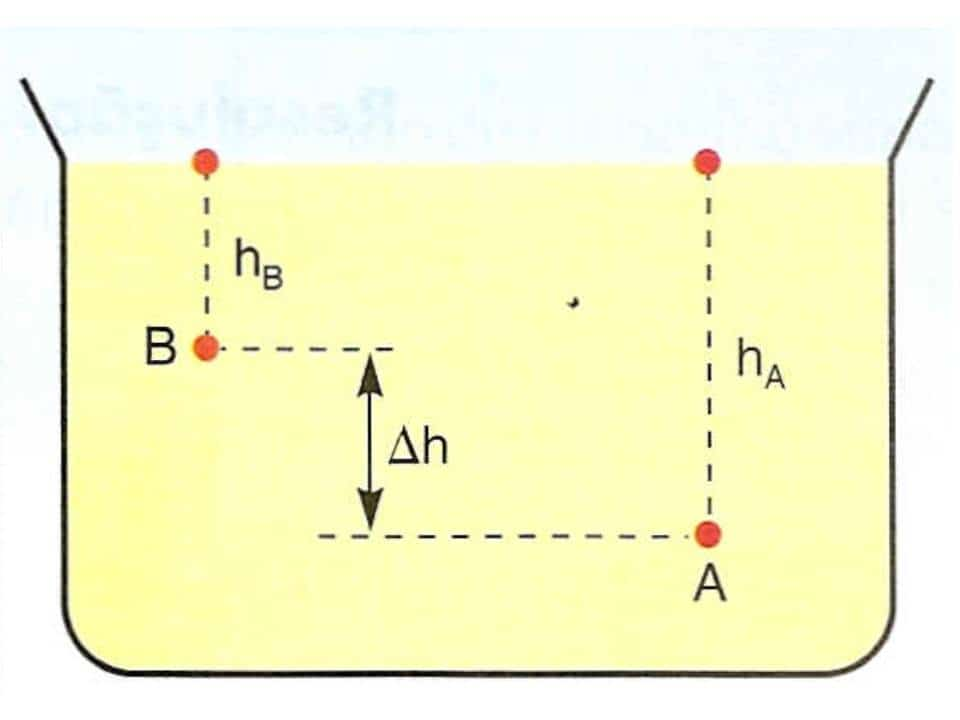
\includegraphics[width=0.6\textwidth]{teorema-de-stevin-1.jpg}
    \caption{Ilustração do Teorema de Stevin.}
    \label{fig:stevin}
\end{figure}

Com isso, a pressão num certo dado ponto do fluído é dado por:
\begin{equation}
    p(h) = p_{atm} + d_{fluido}\,g\,h
\end{equation}
\noindent em que '$p_{atm}$' é a pressão da atmosfera sobre a superfície livre (que na figura acima, é a superfície superior) do fluído, '$d_{fluido}$' é a densidade do fluído, 'g' é a aceleração da gravidade e 'h' é a altura da coluna do fluído, contada a partir da superfície livre.

\textit{Exemplo:} Sabendo que a pressão atmosférica é, aproximadamente, $1.10^5\,Pa$, calcule a altura da coluna de água para que a pressão sobre um mergulhador seja o dobro da pressão atmosférica. \textit{Dados:} $g=10\,m/s^2$ e $d = 10^3\,kg/m^3$.

Usando a fórmula da pressão:
\begin{equation}
    \begin{split}
        &p(h) = p_{atm} + d\,g\,h\\
        &2p_{atm} = p_{atm} + d\,g\,h\\
        &p_atm = d\,g\,h
    \end{split}
\end{equation}
Substituindo os valores:
\begin{equation}
    10^5 = 10^3\,10\,h \implies h = \frac{10^5}{10^4} \implies \boxed{h=10\,m}
\end{equation}

Ou seja, a cada 10 metros de profundidade, a pressão sobre um mergulhador aumenta 1 pressão atmosférica sobre ele. É por isso que, em mergulhos profundos, os mergulhadores não podem subir de uma vez só, eles tem que para a certas alturas, para que o corpo vá se adaptando à diferença de pressão imposta sobre ele.

Uma outra questão interessante sobre o Teorema de Stevin é sobre um conjunto que possui \textbf{vasos comunicantes}: um recipientes com diversas entradas e saídas:
\begin{figure}[H]
    \centering
    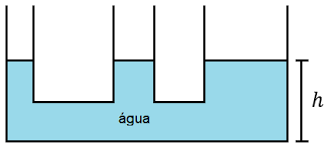
\includegraphics[width=0.6\textwidth]{vasos_comunicantes.png}
    \caption{Ilustração de fluído num recipiente com vasos comunicantes.}
    \label{fig:vasos}
\end{figure}

Perceba que os vasos tem diversos diâmetros, mas a altura da água é a mesma. O mais importante dessa parte é perceber que os tubos que comunicam os vasos não se afinam ou se enlargam. Veremos na aula seguinte, que caso aconteça isso, tem outro princípio que explica o que acontece.

\section{Teorema de Pascal}
O teorema de Pascal diz o seguinte: em tubo fechado com um fluído, a pressão aplicada numa extremidade é transmitida de forma integral até a outra extremidade do fluído. Ou seja, a pressão aplicada num ponto do fluído aparece na outra parte do fluído de forma igual.

De forma matemática, isso se traduz:
\begin{equation}
    p_1 = p_2
\end{equation}
\noindent em que '$p_1$' é a pressão numa extremidade e '$p_2$' é a pressão na outra extremidade.

Pela equação (\ref{eq:pressao}), reescrevemos como:
\begin{equation}
    \frac{F_1}{A_1} = \frac{F_2}{A_2}
\end{equation}
\noindent em que $F_1,\,A_1$ são a força aplicada e a Área de contato da extremidade 1 e $F_2,\,A_2$ são a força e a área de contato na extremidade 2. A figura abaixo exemplifica isso:
\begin{figure}[H]
    \centering
    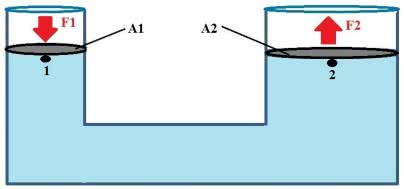
\includegraphics[width=0.6\textwidth]{mbolos.jpg}
    \caption{Ilustração do Teorema de Pascal}
    \label{fig:pascal}
\end{figure}

Perceba que, para o caso $A_1 < A_2$ (como na figura), quando eu aplico uma força na extremidade 1, a força $F_2$ será maior do que a força $F_1$:
\begin{equation}
    \frac{F_1}{A_1} = \frac{F_2}{A_2} \implies F_2 = \frac{A_2}{A_1}\,F_1
\end{equation}

Esse é o princípio das bombas hidraulicas, dos elevadores de carro, das antigas cadeiras de dentista\footnote{As cadeiras mais modernas são a base de motores elétricos e pistões pneumáticos (a base de bombas de ar).}. Porém, a sua maior utilidade é nos freios de carros, em que o pedal de freio que o motorista aperta é a extremidade 1 e a força aplicada para freiar é a força $F_2$.

\begin{figure}[H]
    \centering
    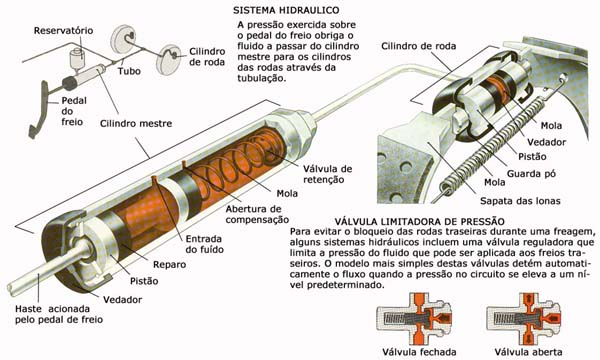
\includegraphics[width=0.9\textwidth]{Válvula-limitadora-de-pressão.jpg}
    \caption{Infográfico de explicação dos componentes do sistema de freios de um carro. O Teorema de Pascal se aplica no pistão que está acoplado ao pedal de freio.}
    \label{fig:freio}
\end{figure}

\textit{Exemplo}: Dado um elevador hidraulico em que queremos levantar um carro de 1 tonelada (1000 kg). A área de contato em que o carro toca o elevador é de 5 $m^2$. Supondo que a outra extremidade onde se aplica a força tem áre de 0,025 $m^2$, qual é a força miníma a ser aplicada para que o carro seja levantado? \textit{Note e adote: $g=10\,m/s^2$}.

Existem 2 forças envolvidas no carro: a força peso (P) e a força aplicada pelo elevador para subir ($F_2$). A força mínima ($F_2$) para que o carro suba é aquela que iguala a força peso:
\begin{equation}
    F_2 = P \implies F_2 = 10*10^3 \implies F_2 = 10^4\, N
\end{equation}

Com isso, usando o Teorema de Pascal:
\begin{equation}
    \frac{F_1}{A_1} = \frac{F_2}{A_2} \implies F_1 = \frac{A_1}{A_2}F_2
\end{equation}
Colocando os dados:
\begin{equation}
    F_1 = \frac{0,025}{5}10^4 = \frac{25}{5}*10^{-3}*10^4 \implies F_1 = 5*10^1 \implies F_1 = 50\,N
\end{equation}
Ou seja, basta uma força maior que 50 N aplicada na extremidade do elevador para que o carro seja levantado.

\section{Teorema de Arquimedes - Empuxo}

O Teorema de Arquimedes é um dos mais antigos teoremas físicos que sua validade ainda sobreviveram até hoje. A história desse teorema é uma das mais interessantes e o brilhantismo de Arquimedes transparece nela. O Rei Hierão II, rei de Siracusa, chamou Arquimedes para uma missão: desconfiado de seu ferreiro, chamou Arquimedes para investigar se sua coroa era feita de uma mistura de ouro e prata ou se era feita inteiramente de ouro.

Mas para isso, o desafio era descobrir isso, sem ter que derreter a coroa. Enquanto pensava no problema, Arquimedes foi tomar um banho numa banheira e durante o banho descobriu a solução. Ele saiu pelas ruas correndo nu gritando '\textit{Eureka}', '\textit{Eureka}'.

O que Arquimedes descobriu foi que quando ele mergulhava na banheira, o nível de água dela se descolava. Mas não era qualquer quantidade, \textbf{o volume de água deslocado era igual ao volume do corpo mergulhado.} Então, Arquimedes resolveu o problema da seguinte forma: Ele encheu totalmente uma banheira com água e mergulhou a coroa. O nível d'água desloca, transborda da banheira e ele recolhe essa água que transbordou, medindo o seu volume.

Naquela época, o gregos já tinham o conhecimento sobre densidade dos metais, então, comparando a massa da coroa com o volume de água transbordada, ele descobriu que a densidade da coroa não condizia com a densidade do ouro. Portanto, a coroa era feita com uma mistura de prata e ouro.

Além disso, Arquimedes percebeu que quando submergimos uma objeto na água (ou em qualquer líquido), ele aparenta estar mais leve, é como se a água ajudasse a sustentar o objeto. Essa força vertical para cima que o líquido exerce no objeto submerso é chamada de \textbf{Empuxo ($\vec{E}$)} e ela aparece devido à diferença de pressão entre as faces inferiores e superiores do objeto.

O Empuxo é descrito pela seguinte fórmula:
\begin{equation}
    E = d_{fluido}\,g\,V_{sub}
\end{equation}
\noindent em que $d_{fluido}$ é a densidade do fluído, $g$ é a aceleração da gravidade e $V_{sub}$ é o volume do objeto que tá submerso no fluído.
\begin{figure}[H]
    \centering
    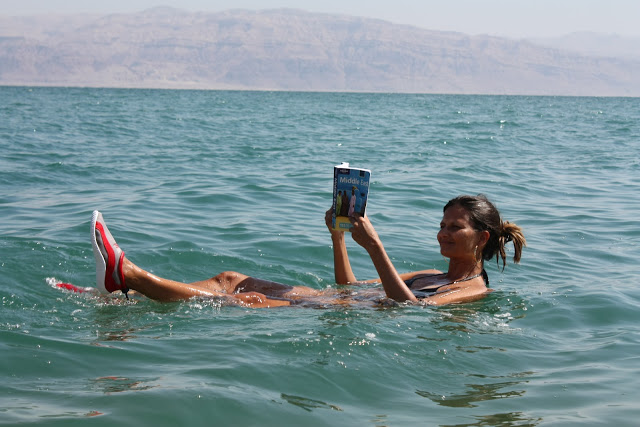
\includegraphics[width=0.6\textwidth]{mar_morto.JPG}
    \caption{Um dos exemplos mais clássicos sobre o Empuxo é o flutuar no Mar Morto - um lago no interior de Israel que possui uma concentração de sal extremamente grande. Por causa disso, a densidade da água é bem maior que a densidade da água do mar e dessa forma, fica bem fácil de flutuar e difícil de mergulhar.}
    \label{fig:mar_morto}
\end{figure}

\section{Vazão e Equação da Continuidade}
A vazão é um conceito de Mecânica dos Fluídos que descreve o quanto de volume de um fluído passa por uma área A num intervalo de tempo:
\begin{equation}
    \phi = \frac{\Delta V}{\Delta t}
\end{equation}
\noindent em que $\phi$ é a vazão e $\Delta V$ é o quanto de água passou no intervalo de tempo $\Delta t$. A unidade do SI é \textbf{metro cúbico por segundo} ($m^3/s$).

Se o tubo for cilíndrico com uma área de seção transversal A e o fluído percorre uma distância $\Delta s$ dentro do tubo, então $\Delta V = A\,\Delta s$:
\begin{equation}
    \phi = \frac{\Delta V}{\Delta t} = \frac{A\,\Delta s}{\Delta t} = A\,v
\end{equation}
\noindent em que 'v' é a velocidade de escoamento do fluído.

Com a vazão, temos uma importante equação: \textbf{A Equação da Continuidade}. Ela diz que para \textbf{fluídos incompressíveis}, tipo a água, \textbf{o fluxo do fluído ($\phi$) dentro de um tubo tem que ser um valor constante, não importando se esse tubo muda de diâmetro ou formato}. 

Ou seja, para um caso que o tubo inicialmente tenha uma área de seção $A_1$ e depois passa a ter uma área de seção $A_2$, a relação que conecta essas 2 quantidades é:
\begin{equation}
    \phi_1=\phi_2 \implies A_1\,v_1 = A_2\,v_2
\end{equation}
\noindent em que $v_1,\,v_2$ são a velocidade de escoamento do fluído.
\begin{figure}[H]
    \centering
    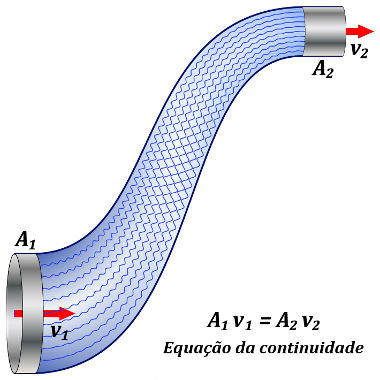
\includegraphics[width=0.4\textwidth]{equacao-continuidade.jpg}
    \caption{Esquema sobre a Equação da Continuidade}
    \label{fig:eq_continuidade}
\end{figure}

Essa relação fala que se o tubo possui um estrangulamento, ou seja, o diâmetro do tubo diminui, a velocidade de escoamento aumenta para que mantenha o fluxo constante. É por causa disso que uma forma de fazer a água chegar mais longe e/ou sair com mais velocidade de uma mangueira, nós tapamos uma parte da saída da mangueira.
\begin{figure}[H]
    \centering
    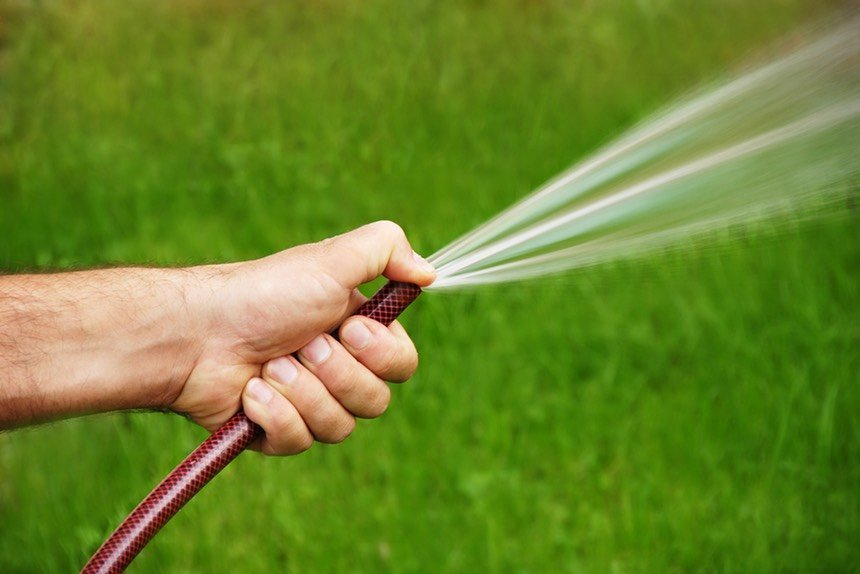
\includegraphics[width=0.6\textwidth]{pressao-agua.jpeg}
    \caption{Quando tapamos uma parte da saída da mangueira, a água sai com mais velocidade e pressão, indo mais longe}
    \label{fig:eq_continuidade}
\end{figure}

Outra questão interessante é sobre a água saindo da torneira. Se abrirmos a torneira, vemos que o jato de água vai afunilando. Por que isso acontece?

Isso é devido à gravidade que acelera a água. Como a água ganha a velocidade, pela Equação da Continuidade, a área que o jato ocupa tem que diminuir para que a vazão seja a mesma. É por isso que o jato de água fica menor conforme ela vai caindo na pia.

\section{Equação de Bernoulli}
Daniel Bernoulli, um dos físicos da brilhante família de físicos Bernoulli, descreveu uma equação que é uma das mais importantes para a Mecânica dos Fluídos: a \textbf{Equação de Bernoulli}:
\begin{equation}
    p_1 + dg\,h_1 + \frac{d\,v_1^2}{2} = p_2 + dg\,h_2 + \frac{d\,v_2^2}{2}
\end{equation}
\noindent em que os subescritos 1,2 são 2 pontos de interesse dentro de um tubo ou espaço onde um fluído esteja passando, 'p' é a pressão que esse fluído está submetido, 'd' é a densidade, 'h' é a altura em relação a um ponto de interesse e 'v' é a velocidade de escoamento.
\begin{figure}[H]
    \centering
    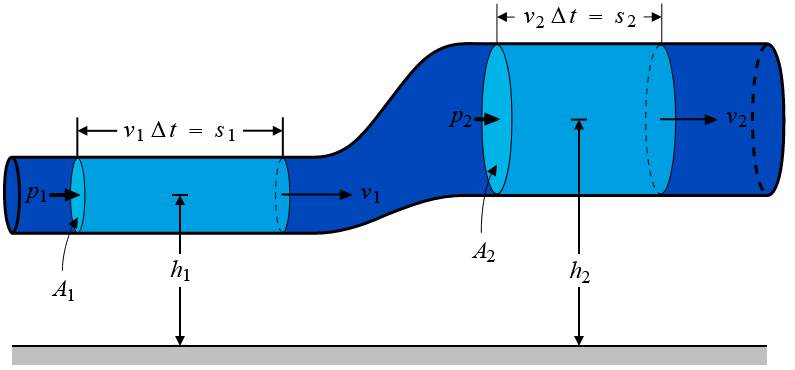
\includegraphics[width=0.6\textwidth]{principio_bernoulli.png}
    \caption{Esquema do Princípio de Bernoulli - quando o fluído passa pelo}
    \label{fig:Bernoulli}
\end{figure}

É por causa dessa Equação de Bernoulli que quando estamos na praia e entramos numa rua/avenida que tem prédios altos, a brisa do mar fica mais forte. Como basicamente, a altura entre a praia e a rua é a mesma, então a velocidade do vento aumenta e a pressão diminui.

Com as 2 equações (da Continuidade e de Bernoulli) conseguimos descrever sistemas bem complexos e áreas muito importantes foram desenvolvidas como a Aerodinâmica. Ela está presente na engenharia aeronaútica, na construção dos aviões, em especial, na construção das asas dos aviões:

\begin{figure}[H]
    \centering
    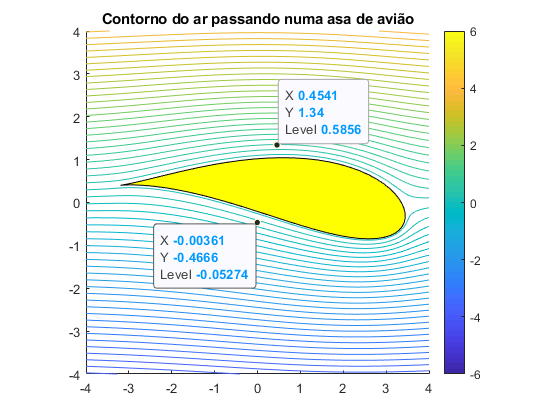
\includegraphics[width=0.8\textwidth]{asa_de_aviao.png}
    \caption{Esquema dos caminhos que o ar faz quando passa por uma asa de Avião. Perceba que o valor por cima da asa é maior que por baixo. Isso significa que o ar anda mais rápido por cima do que por baixo, logo a pressão em baixo da asa é maior que em cima, criando a força de sustentação}
    \label{fig:asa_aviao}
\end{figure}
\end{document}
